\documentclass[12pt]{article}
\usepackage{lecture}
\usepackage{graphics}
\usepackage{html}
\usepackage{url}
\usepackage{epstopdf}

\newcommand{\copyrightYears}{2001-2021}

\title{Introduction to quantitative genetics}

\begin{document}

\maketitle

\thispagestyle{first}

So far in this course we have dealt entirely either with the evolution
of characters that are controlled by simple Mendelian inheritance at a
single locus or with the evolution of molecular sequences. Even last
week when we were dealing with population genomic data, data from
hundreds or thousands of loci, we were treating the variation at each
locus separately and combining results across loci. I have some old
notes on gametic disequilibrium and how allele frequencies change at
two loci simultaneously, but they're in the ``Old notes, no longer
updated'' section of the book version of these
notes~(\url{https://figshare.com/articles/journal_contribution/Lecture_notes_in_population_genetics/100687}),
and we didn't discuss them.\footnote{We will spend some time talking
  about gametic disequilibrium when we talk about association mapping
  in a couple of weeks.} In every example we've considered so far
we've imagined that we could understand something about evolution by
examining the evolution of a single gene. That's the domain of
classical population genetics.

For the next few weeks we're going to be exploring a field that's
older than classical population genetics, although the approach we'll
be taking to it involves the use of population genetic
machinery.\footnote{In fact, it involves the use of the single-locus
  population genetic machinery we've been using all semester.} If you
know a little about the history of evolutionary biology, you may know
that after the rediscovery of Mendel's work in 1900 there was a heated
debate between the ``biometricians'' (e.g., Galton and Pearson) and
the ``Mendelians'' (e.g., de Vries, Correns, Bateson, and
Morgan).\index{biometricians}\index{Mendelians}

Biometricians asserted that the really important variation in
evolution didn't follow Mendelian rules. Height, weight, skin color,
and similar traits seemed to

\begin{itemize}

\item vary continuously,

\item show blending inheritance, and

\item show variable responses to the environment.

\end{itemize}

\noindent Since variation in such {\it quantitative traits\/} seemed
to be more obviously related to organismal adaptation than the
``trivial'' traits that Mendelians studied, it seemed obvious to the
biometricians that Mendelian geneticists were studying a phenomenon
that wasn't particularly interesting.\index{quantitative traits}\index{blending inheritance}

Mendelians dismissed the biometricians, at least in part, because they
seemed not to recognize the distinction between genotype and
phenotype. It seemed to at least some Mendelians that traits whose
expression was influenced by the environment were, by definition, not
inherited. Moreover, the evidence that Mendelian principles accounted
for the inheritance of many discrete traits was incontrovertible.

Woltereck's~\cite{Woltereck-1909} experiments on {\it Daphnia\/}
helped to show that traits whose expression is environmentally
influenced may also be inherited. He introduced the idea of a {\it
  norm of reaction} to describe the observation that the same genotype
may produce different phenotypes in different
environments~(Figure~\ref{fig:norm-of-reaction}). When you fertilize a
plant, for example, it will grow larger and more robust than when you
don't. The phenotype an organism expresses is, therefore, a product of
{\it both\/} its genotype and its environment.\index{norm of reaction}\index{phenotypic plasticity}

\begin{figure}
\begin{center}
\resizebox{!}{6cm}{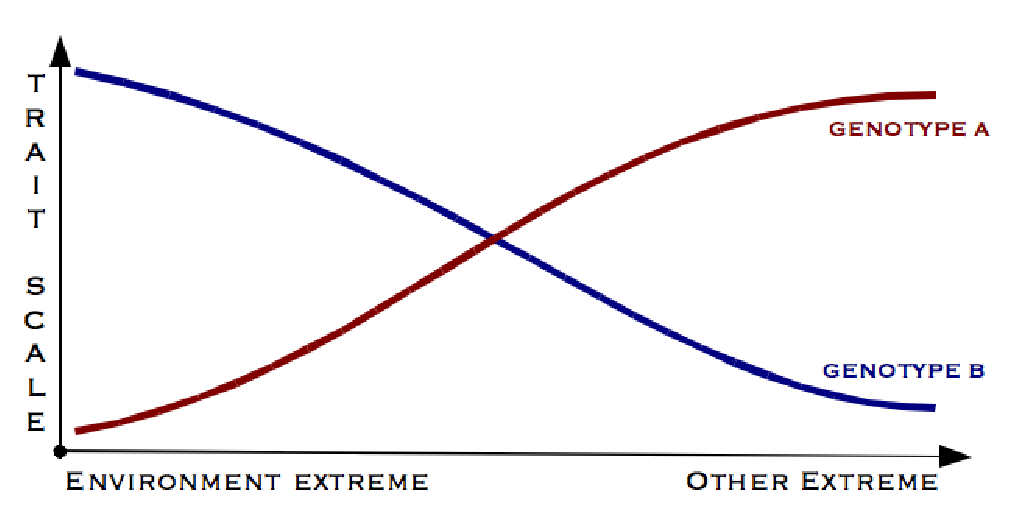
\includegraphics{Trait-scale-linear.eps}}
\end{center}
\caption{Hypothetical illustration of reaction norms for two genotypes
  across a 1-dimensional environmental gradient~(from Wikipedia,
  Public Domain,
  {\tt https://en.wikipedia.org/w/index.php?curid=3925138}, accessed 9
  April 2017).}\label{fig:norm-of-reaction}
\end{figure}

Nilsson-Ehle's~\cite{NilssonEhle-1909} experiments on inheritance of
kernel color in wheat showed how continuous variation and Mendelian
inheritance could be reconciled~(Figure~\ref{fig:nilsson-ehle}). He
demonstrated that what appeared to be continuous variation in color
from red to white with blending inheritance could be understood as the
result of three separate genes influencing kernel color that were
inherited separately from one another. It was the first example of
what's come to be known as {\it polygenic inheritance}. Fisher~\cite{Fisher-1918}, in a paper that grew out of
his undergraduate Honors thesis at Cambridge University, set forth the
mathematical theory that describes how it all works. That's the theory
of {\it quantitative genetics}, and it's what we're going to spend the
next several weeks discussing.\index{polygenic inheritance}

\begin{figure}
\begin{center}
\resizebox{!}{10cm}{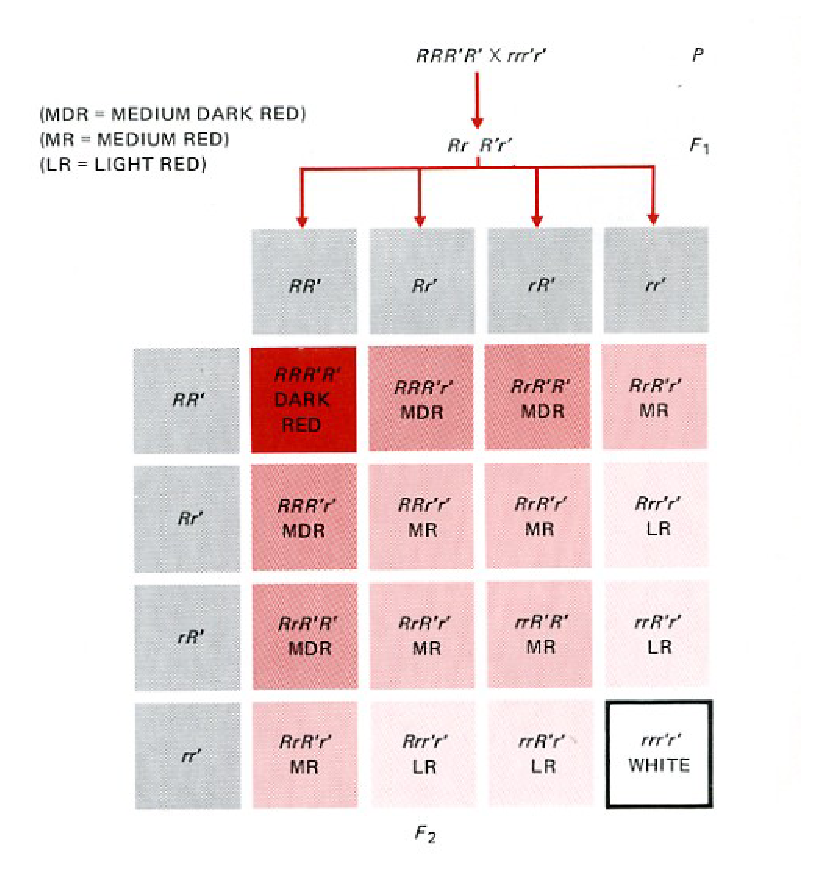
\includegraphics{Nilsson-Ehle.eps}}
\end{center}
\caption{Results from one of Nilsson-Ehle's crosses illustrating
  polygenic inheritance of kernel color in wheat~(from {\tt
    http://www.biology-pages.info/Q/QTL.html}, accessed 9 April 2017).}\label{fig:nilsson-ehle}
\end{figure}

\section*{An overview of where we're headed}

Woltereck's ideas force us to realize that when we see a phenotypic
difference between two individuals in a population there are three
possible sources for that difference:

\begin{enumerate}

\item The individuals have different genotypes.

\item The individuals developed in different environments.

\item The individuals have different genotypes {\it and\/} they
developed in different environments.

\end{enumerate}

\noindent This leads us naturally to think that phenotypic variation
consists of two separable components, namely genotypic and
environmental components.\footnote{We'll soon see that separating
  genotypic and environmental components is far from trivial. I'm also
  putting aside, for the moment, that genotypes may differ in their
  response to the environment, even though that's what I illustrated
  in discussing norms of reaction.} Putting that into an equation
\[
\Var(P) = \Var(G) + \Var(E) \quad ,
\]
where $\Var(P)$ is the {\it phenotypic variance}, $\Var(G)$ is the
{\it genetic variance}, and $\Var(E)$ is the environmental
variance.\footnote{Strictly speaking we should also include a term for
  the interaction between genotype and environment, but we'll ignore
  that for the time being. I illustrated the interaction between
  genotype and environment in discussing norms of reaction.} As
we'll see in just a moment, we can also partition the genetic variance
into components, the {\it additive genetic variance\/}, $\Var(A)$, and
the {\it dominance variance}, $\Var(D)$.\footnote{We could even
  partition it further into additive by additive, additive by
  dominance, and dominance by dominance epistatic variance, but let's
  not go there.}\index{phenotypic variance!partitioning}\index{genetic
  variance}\index{environmental variance}

There's a surprisingly subtle and important insight buried in that
very simple equation: Because the expression of a quantitative trait
is a result both of genes involved in that trait's expression and the
environment in which it is expressed, it doesn't make sense to say of
a particular individual's phenotype that genes are more important than
environment in determining it. You wouldn't have a phenotype without
both. At most what we can say is that when we look at a particular
population of organisms some fraction of the phenotypic variation they
exhibit is due to differences in the genes they carry and that some
fraction is due to differences in the environment they have
experienced.\footnote{When I put it this way, I hope it's obvious that
  I'm neglecting genotype-environment interactions, and that I'm
  oversimplifying a lot.}\index{nature vs.\ nurture} If we have two
individuals with different phenotypes, e.g., Ralph is tall and Harry
is short, we can't even say whether the difference between Ralph and
Harry is because of differences in their genes or differences in their
developmental environment.

One important implication of this insight is that much of the ``nature
vs.\ nurture'' debate concerning human intelligence or human
personality characteristics is misguided. The intelligence and
personality that you have is a product of {\it both} the genes you
happened to inherit and the environment that you happened to
experience. Any differences between you and the person next to you
probably reflect both differences in genes {\it and\/} differences in
environment. Moreover, even if the differences between you and your
neighbor are due to differences in genes, it doesn't mean that those
differences are fixed and indelible. You may be able to do something
to change them.

Take phenylketonuria, for example. It's a condition in which
individuals are homozygous for a deficiency that prevents them from
metabolizing
phenylalanine~(\url{https://medlineplus.gov/phenylketonuria.html}).
If individuals with phenylketonuria eat a normal diet, severe
intellectual disabilities can result by the time an infant is one year
old. But if they eat a diet that is very low in phenylalanine, their
development is completely normal.\index{phenylketonuria} In other
words, clear genetic differences at this locus {\it can\/} lead to
dramatic differences in cognitive ability, but {\it they don't have
  to}.

It's often useful to talk about how much of the phenotypic variance is
a result of additive genetic variance or of genetic variance.
\[
h^2_n = \frac{\Var(A)}{\Var(P)}
\]
is what's known as the {\it narrow-sense heritability}. It's the
proportion of phenotypic variance that's attributable to differences
among individuals in their additive genotype,\footnote{Don't worry
  about what I mean by {\it additive genotype}{\dash}yet. We'll get to
  it soon enough.} much as $F_{st}$ can be thought of as the
proportion of genotypic diversity that attributable to differences
among populations.\index{heritability!narrow sense} Similarly,
\[
h^2_b = \frac{\Var(G)}{\Var(P)}
\]
is the {\it broad-sense heritability}. It's the proportion of
phenotypic variance that's attributable to differences among
individuals in their genotype. It is {\it not}, repeat {\bf\it NOT}, a
measure of how important genes are in determining phenotype. Every
individuals phenotype is determined both by its genes and by its
phenotype. It measures how much of the {\it difference\/} among
individuals is attributable to differences in their genes.\footnote{As
  we'll see later it can do this only for the range of environments in
  which it was measured.}\index{heritability!broad sense} Why bother
to make the distinction between narrow- and broad-sense heritability?
Because, as we'll see, it's only the additive genetic variance that
responds to natural selection.\footnote{Or at least only the additive
  genetic variance responds to natural selection when zygotes are
  found in Hardy-Weinberg proportions.} In fact,
\[
R = h^2_nS \quad ,
\]
where $R$ is the {\it response to selection\/} and $S$ is the
{\it selective differential}.\index{response to selection}

As you'll see in the coming weeks, there's a lot of stuff hidden
behind these simple equations, including a lot of assumptions. But
quantitative genetics is very useful. Its principles have been widely
applied in plant and animal breeding for more than a century, and they
have been increasingly applied in evolutionary investigations in the
last forty years.\footnote{I used to include a joke here that I've
  decided not to include any more. It's not very funny, and some
  people might find it offensive. If for some reason you want to know
  what the joke is, you can find it in the 2017 version of these notes
  on Figshare~(\url{https://doi.org/10.6084/m9.figshare.100687.v2})}.

\section*{Partitioning the phenotypic variance}

Before we worry about how to estimate any of those variance components
I just mentioned, we first have to understand what they are. So let's
start with some
definitions~(Table~\ref{table:definitions}).\footnote{Warning! There's
  a {\it lot\/} of algebra and even a little differential calculus
  between here and the end. It's unavoidable. You can't possibly
  understand what additive genetic variance is without it. I'll try to
  focus on principles, and I'll do my best to keep reminding us all
  why we're slogging through the math, but a lot of the math that
  follows {\it is\/} necessary. Sorry about that.}

\begin{table}
\begin{center}
\begin{tabular}{l|ccc}
\hline\hline
Genotype                 & $A_1A_1$    & $A_1A_2$ & $A_2A_2$ \\
\hline
Frequency                & $p^2$       & $2pq$    & $q^2$ \\
Genotypic value          & $x_{11}$    & $x_{12}$ & $x_{22}$ \\
Additive genotypic value & $2\alpha_1$ & $\alpha_1 + \alpha_2$
                                                  & $2\alpha_2$ \\
\hline
\end{tabular}
\end{center}
\caption{Fundamental parameter definitions for quantitative genetics
  with one locus and two alleles.}\label{table:definitions}
\end{table}\index{genotypic value}\index{additive genotypic value}\index{genotypic value!additive}

You should notice something rather strange about
Table~\ref{table:definitions} when you look at it. I motivated the
entire discussion of quantitative genetics by talking about the need
to deal with variation at many loci, and what I've presented involves
only two alleles at a single locus. I do this for two reasons:

\begin{enumerate}

\item It's not too difficult to do the algebra with multiple alleles
  at one locus instead of only two, but it gets messy, doesn't add any
  insight, and I'd rather avoid the mess.

\item Doing the algebra with multiple loci involves a {\it lot\/} of
  assumptions, which I'll mention when we get to applications, and the
  algebra is even worse than with multiple alleles.

\end{enumerate}

\noindent Fortunately, the basic principles extend with little
modification to multiple loci, so we can see all of the underlying
logic by focusing on one locus with two alleles where we have a chance
of understanding what the different variance components mean.

Two terms in Table~\ref{table:definitions} will almost certainly be
unfamiliar to you: {\it genotypic value\/} and {\it additive genotypic
  value}. Of the two, {\it genotypic value\/} is the easiest to
understand~(Figure~\ref{fig:genotypic-value}). It simply refers to the
average phenotype associated with a given
genotype.\footnote{Remember. We're now considering traits in which the
  environment influences the phenotypic expression, so the same
  genotype can produce different phenotypes, depending on the
  environment in which it develops.} The {\it additive genotypic
  value\/} refers to the average phenotype associated with a given
genotype, as would be inferred from the {\it additive effect\/} of the
alleles of which it is composed. That didn't help much, did it? That's
because I now need to tell you what we mean by the {\it additive
  effect\/} of an allele.\footnote{Hold on. Things get even more
  interesting, i.e., worse from here.}

\begin{figure}
\begin{center}
\resizebox{!}{7cm}{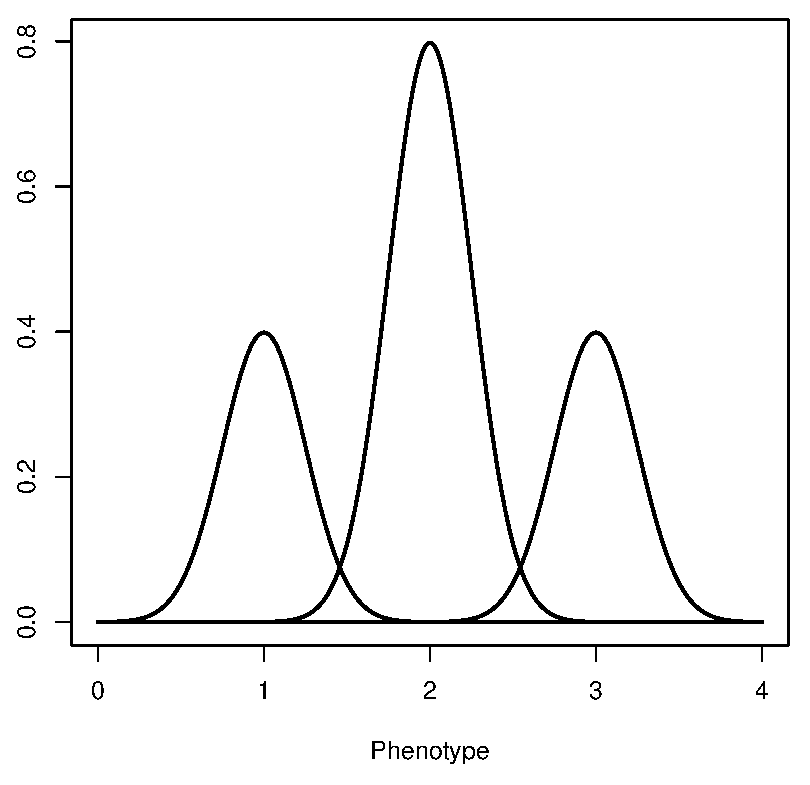
\includegraphics{genotypic-value.eps}}
\end{center}
\caption{The phenotype distribution in a population in which the three
  genotypes at a single locus with two alleles occur in Hardy-Weinberg
  proportions and the alleles occur in equal frequency. The $A_1A_1$
  genotype has a mean trait value of 1, the $A_1A_2$ genotype has a
  mean trait value of 2, and the $A_2A_2$ genotype has a mean trait
  value of 3, but each genotype can produce a range of phenotypes with
  the standard deviation of the distribution being 0.25 in each
  case.}\label{fig:genotypic-value}
\end{figure}

\subsection*{The additive effect of an allele}\index{additive effect}

In constructing Table~\ref{table:definitions} I used the quantities
$\alpha_1$ and $\alpha_2$, but I didn't tell you where they came
from. Obviously, the idea should be to pick values of $\alpha_1$ and
$\alpha_2$ that give additive genotypic values that are reasonably
close to the genotypic values. A good way to do that is to minimize
the squared deviation between the two, weighted by the frequency of
the genotypes. So our first big assumption is that genotypes are in
Hardy-Weinberg proportions.\footnote{As you should have noticed in
  Table~\ref{table:definitions}.}\index{additive effect!Hardy-Weinberg assumption}

The objective is to find values for $\alpha_1$ and $\alpha_2$ that
minimize:
\[
a = p^2[x_{11}-2\alpha_1]^2
       + 2pq[x_{12}-(\alpha_1+\alpha_2)]^2
       + q^2[x_{22}-2\alpha_2]^2 \quad .
\]
To do this we take the partial derivative of $a$ with respect to both
$\alpha_1$ and $\alpha_2$, set the resulting pair of equations equal
to zero, and solve for $\alpha_1$ and $\alpha_2$.\footnote{We won't
  bother with proving that the resulting estimates produce the minimum
  possible value of $a$. Just take my word for it. Or if you don't
  believe me and know a little calculus, take the second partials of
  $a$ and evaluate it with the values of $\alpha_1$ and $\alpha_2$
  substituted in. You'll find that the resulting matrix of partial
  derivatives, the Hessian matrix, is positive definite, meaning that
  we've found values that minimize the value of $a$. If you don't know
  what any of that means, just take my word for it that the values of
  $\alpha_1$ and $\alpha_2$ we get minimize the value of $a$.}
\begin{eqnarray*}
\frac{\partial a}{\partial{\alpha_1}} &=& p^2\{2[x_{11} - 2\alpha_1][-2]\}
                     + 2pq\{2[x_{12} - (\alpha_1+\alpha_2)][-1]\} \\
                  &=& -4p^2[x_{11} - 2\alpha_1]
                     -4pq[x_{12} - (\alpha_1+\alpha_2)] \\
\frac{\partial a}{\partial{\alpha_2}} &=& q^2\{2[x_{22} - 2\alpha_2][-2]\}
                     + 2pq\{2[x_{12} - (\alpha_1+\alpha_2)][-1]\} \\
                  &=& -4q^2[x_{22} - 2\alpha_2]
                     -4pq[x_{12} - (\alpha_1+\alpha_2)]
\end{eqnarray*}
Thus, $\frac{\partial a}{\partial{\alpha_1}} = \frac{\partial a}{\partial{\alpha_2}} = 0$ if and only if
\begin{eqnarray}
p^2(x_{11} - 2\alpha_1) + pq(x_{12} - \alpha_1 - \alpha_2) &=& 0
  \nonumber \\
q^2(x_{22} - 2\alpha_2) + pq(x_{12} - \alpha_1 - \alpha_2) &=& 0
\label{eq:zeros}
\end{eqnarray}
Adding the equations in~(\ref{eq:zeros}) we obtain (after a little bit
of rearrangement)
\begin{equation}
[p^2x_{11} + 2pqx_{12} + q^2x_{22}] -
   [p^2(2\alpha_1) + 2pq(\alpha_1 + \alpha_2) + q^2(2\alpha_2)] = 0 \quad .
\label{eq:basic}
\end{equation}

Now the first term in square brackets is just the mean phenotype in
the population, $\bar x$.  Thus, we can rewrite
equation~(\ref{eq:basic}) as:
\begin{eqnarray}
{\bar x} &=& 2p^2\alpha_1 + 2pq(\alpha_1 + \alpha_2)
                        +2q^2\alpha_2 \nonumber \\
                     &=& 2p\alpha_1(p+q) + 2q\alpha_2(p+q) \nonumber \\
                     &=& 2(p\alpha_1 + q\alpha_2) \quad . \label{eq:alpha_bar}
\end{eqnarray}
Now divide the first equation in (\ref{eq:zeros}) by $p$ and the
second by $q$.
\begin{eqnarray}
p(x_{11} - 2\alpha_1) + q(x_{12} - \alpha_1 - \alpha_2) &=& 0
\label{eq:zeros_divide_1} \\
q(x_{22} - 2\alpha_2) + p(x_{12} - \alpha_1 - \alpha_2) &=& 0 \quad
. \label{eq:zeros_divide_2}
\end{eqnarray}
Thus,
\begin{eqnarray*}
px_{11} + qx_{12} &=& 2p\alpha_1 + q\alpha_1 + q\alpha_2 \\
 &=& \alpha_1(p + q) + p\alpha_1 + q\alpha_2 \\
 &=& \alpha_1 + p\alpha_1 + q\alpha_2 \\
 &=& \alpha_1 + {\bar x}/2 \\
\alpha_1 &=& px_{11} + qx_{12} - {\bar x}/2 \quad .
\end{eqnarray*}
Similarly,
\begin{eqnarray*}
px_{12} + qx_{22} &=& 2q\alpha_2 + p\alpha_1 + p\alpha_2 \\
 &=& \alpha_2(p + q) + p\alpha_1 + q\alpha_2 \\
 &=& \alpha_2 + p\alpha_1 + q\alpha_2 \\
 &=& \alpha_2 + {\bar x}/2 \\
\alpha_2 &=& px_{12} + qx_{22} - {\bar x}/2 \quad .
\end{eqnarray*}
$\alpha_1$ is the additive effect of allele $A_1$, and $\alpha_2$ is
the additive effect of allele $A_2$. If we use these expressions, the
additive genotypic values are as close to the genotypic values as
possible, given the particular allele frequencies in the
population.\footnote{If you've been paying close attention and you
  have a good memory, the expressions for $\alpha_1$ and $\alpha_2$
  may look vaguely familiar. They look a lot like the expressions for
  marginal fitnesses we encountered when studying viability
  selection.}\index{additive effect}

\subsection*{Components of the genetic variance}\index{genetic variance!components}

Let's assume for the moment that we can actually measure the genotypic
values. Later, we'll relax that assumption and see how to use the
resemblance among relatives to estimate the genetic components of
variance. But it's easiest to see where they come from if we assume
that the genotypic value of each genotype is known. If it is then,
writing $V_g$ for $\Var(G)$
\begin{eqnarray}
V_g &=&\ p^2[x_{11} - {\bar x}]^2 + 2pq[x_{12} - {\bar x}]^2
     + q^2[x_{22} - {\bar x}]^2 \label{eq:v-g} \\
    &=&\ p^2[x_{11} - 2\alpha_1 + 2\alpha_1 - {\bar x}]^2
     + 2pq[x_{12} - (\alpha_1 + \alpha_2) + (\alpha_1 + \alpha_2)
                - {\bar x}]^2 \nonumber \\
     &&\ \ + q^2[x_{22} - 2\alpha_2 + 2\alpha_2 - {\bar x}]^2
     \nonumber \\
    &=&\ p^2[x_{11} - 2\alpha_1]^2 + 2pq[x_{12} - (\alpha_1+\alpha_2)]^2
       + q^2[x_{22} - 2\alpha_2]^2 \nonumber \\
     &&\ + p^2[2\alpha_1 - {\bar x}]^2 + 2pq[(\alpha_1 + \alpha_2) - {\bar x}]^2
       + q^2[2\alpha_2 - {\bar x}]^2 \nonumber \\
     &&\ + p^2[2(x_{11} - 2\alpha_1)(2\alpha_1 - {\bar x})]
       +2pq[2(x_{12} - \{\alpha_1+\alpha_2\})(\{\alpha_1+\alpha_2\} -
     {\bar x})] \nonumber \\
     &&\ +q^2[2(x_{22} - 2\alpha_2)(2\alpha_2 - {\bar x})] \quad .
     \label{eq:part-begin}
\end{eqnarray}
There are two terms in~(\ref{eq:part-begin}) that have a biological
(or at least a quantitative genetic) interpretation.  The term on the
first line is the average squared deviation between the genotypic
value and the additive genotypic value.  It will be zero only if the
effects of the alleles can be decomposed into strictly additive
components, i.e., only if the phenotype of the heterozygote is exactly
intermediate between the phenotype of the two homozygotes.  Thus, it
is a measure of how much variation is due to non-additivity
(dominance) of allelic effects.  In short, the {\it dominance genetic
variance}, $V_d$, is\index{dominance genetic variance}\index{genetic variance!dominance}
\begin{equation}
V_d = p^2[x_{11} - 2\alpha_1]^2 + 2pq[x_{12} - (\alpha_1+\alpha_2)]^2
          + q^2[x_{22} - 2\alpha_2]^2 \quad .\label{eq:v-d}
\end{equation}
Similarly, the term on the second line of~(\ref{eq:part-begin}) is the
average squared deviation between the additive genotypic value and the
mean genotypic value in the population.  Thus, it is a measure of how
much variation is due to differences between genotypes in their
additive genotype.  In short, the {\it additive genetic variance},
$V_a$, is\index{additive genetic variance}\index{genetic variance!dominance}
\begin{equation}
V_a = p^2[2\alpha_1 - {\bar x}]^2 + 2pq[(\alpha_1 + \alpha_2) - {\bar x}]^2
          + q^2[2\alpha_2 - {\bar x}]^2 \quad .\label{eq:v-a}
\end{equation}
What about the terms on the third and fourth lines of the last
equation in \ref{eq:part-begin}?  Well, they can be rearranged as
follows:
\begin{eqnarray*}
p^2[2(x_{11} &-& 2\alpha_1)(2\alpha_1 - {\bar x})]
 + 2pq[2(x_{12} - \{\alpha_1+\alpha_2\})(\{\alpha_1+\alpha_2\} - {\bar
 x})] \\
 &&+ q^2[2(x_{22} - 2\alpha_2)(2\alpha_2 - {\bar x})] \\
&=& 2p^2(x_{11}-2\alpha_1)(2\alpha_1 - {\bar x})
   + 4pq[x_{12}-(\alpha_1+\alpha_2)][(\alpha_1+\alpha_2)-{\bar x})] \\
 &&+ 2q^2(x_{22}-2\alpha_2)(2\alpha_2 - {\bar x}) \\
&=&\ 4p^2(x_{11}-2\alpha_1)[\alpha_1 - (p\alpha_1+q\alpha_2)] \\
 &&+ 4pq[x_{12}-(\alpha_1+\alpha_2)][(\alpha_1+\alpha_2)-2(p\alpha_1+q\alpha_2)] \\
 &&+ 4q^2(x_{22}-2\alpha_2)[\alpha_2 - (p\alpha_1+q\alpha_2)] \\
&=& 4p[\alpha_1-(p\alpha_1+q\alpha_2)]
      [p(x_{11}-2\alpha_1) + q(x_{12}-\{\alpha_1+\alpha_2\})] \\
 &&+ 4q[\alpha_2-(p\alpha_1+q\alpha_2)]
      [p(x_{11}-2\alpha_1)p + q(x_{12}-\{\alpha_1+\alpha_2\})] \\
&=& 0
\end{eqnarray*}
Where we have used the identities ${\bar x} = 2(p\alpha_1 + q\alpha_2)$ [see
equation~(\ref{eq:alpha_bar})] and
\begin{eqnarray*}
p(x_{11} - 2\alpha_1) + q(x_{12} - \alpha_1 - \alpha_2) &=& 0 \\
q(x_{22} - 2\alpha_2) + p(x_{12} - \alpha_1 - \alpha_2) &=& 0
\end{eqnarray*}
[see equations~(\ref{eq:zeros_divide_1}) and (\ref{eq:zeros_divide_2})].
In short, we have now shown that the total genotypic variance in the
population, $V_g$, can be subdivided into two components{\dash}the
additive genetic variance, $V_a$, and the dominance genetic variance,
$V_d$.  Specifically,
\[
V_g = V_a + V_d \quad ,
\]
where $V_g$ is given by the first line of (\ref{eq:v-g}), $V_a$
by (\ref{eq:v-a}), and $V_d$ by (\ref{eq:v-d}).

\subsection*{An alternative expression for $V_a$}\index{genetic variance!additive}

There's another way to write the expression for $V_a$ when there are
only two alleles at a locus. I show it here because it will come in
handy later.
\begin{eqnarray*}
V_a &=& p^2(2\alpha_1)^2 + 2pq(\alpha_1+\alpha_2)^2 + q^2(2\alpha_2)^2 -
        4(p\alpha_1+q\alpha_2)^2 \\
    &=& 4p^2\alpha_1^2 + 2pq(\alpha_1+\alpha_2)^2 + 4q^2\alpha_2^2
       - 4(p^2\alpha_1^2 +2pq\alpha_1\alpha_2 + q^2\alpha_2^2) \\
    &=& 2pq[(\alpha_1+\alpha_2)^2 - 4\alpha_1\alpha_2] \\
    &=& 2pq[(\alpha_1^2 + 2\alpha_1\alpha_2 + \alpha_2^2) - 4\alpha_1\alpha_2] \\
    &=& 2pq[\alpha_1^2 - 2\alpha_1\alpha_2 + \alpha_2^2] \\
    &=& 2pq[\alpha_1 - \alpha_2]^2 \\
    &=& 2pq\alpha^2 \\
\end{eqnarray*}

\subsection*{An example: the genetic variance with known genotypes}

We've been through a lot of algebra by now. Let's run through a couple
of numerical examples to see how it all works. For the first one,
we'll use the set of genotypic values in Table~\ref{table:additive}.

\begin{table}
\begin{center}
\begin{tabular}{l|ccc}
\hline\hline
Genotype        & $A_1A_1$ & $A_1A_2$ & $A_2A_2$ \\
Genotypic value &  100       & 50        & 0 \\
\hline
\end{tabular}
\end{center}
\caption{A set of perfectly additive genotypic values. Note that the
  genotypic value of the heterozygote is exactly halfway between the
  genotypic values of the two homozygotes.}\label{table:additive}
\end{table}

For $p = 0.4$
\begin{eqnarray*}
{\bar x} &=& (0.4)^2(100) + 2(0.4)(0.6)(50) + (0.6)^2(0) \\
                    &=& 40 \\
\\
\alpha_1 &=& (0.4)(100) + (0.6)(50) - (40)/2 \\
         &=& 50.0 \\
\alpha_2 &=& (0.4)(50) + (0.6)(0) - (40)/2 \\
         &=& 0.0 \\
\\
V_g &=& (0.4)^2(100-40)^2 + 2(0.4)(0.6)(50-40)^2 + (0.6)^2(0-40)^2 \\
    &=& 1200 \\
V_a &=& (0.4)^2[2(50.0)-20]^2 + 2(0.4)(0.6)[(50.0+0.0)-20]^2
       + (0.6)^2[2(0.0)-20]^2 \\
    &=& 1200 \\
V_d &=& (0.4)^2[2(50.0) - 100]^2 + 2(0.4)(0.6)[(50.0+0.0) - 50]^2
       + (0.6)^2[2(0.0) - 0]^2 \\
    &=& 0.00 \quad .
\end{eqnarray*}
For $p = 0.2$, ${\bar x} = 20$, $V_g = V_a = 800$, $V_d = 0.00$.  You
should verify for yourself that $\alpha_1=50$ and $\alpha_2=0$ for
$p=0.2$.  If you are ambitious, you could try to prove that
$\alpha_1=50$ and $\alpha_2=0$ for {\it any\/} allele frequency.

For the second example we'll use the set of genotypic values in
Table~\ref{table:non-additive}.

\begin{table}
\begin{center}
\begin{tabular}{l|ccc}
\hline\hline
Genotype        & $A_1A_1$ & $A_1A_2$ & $A_2A_2$ \\
Genotypic value & 100        & 80      & 0 \\
\hline
\end{tabular}
\end{center}
\caption{A set of non-additive genotypic values. Note that the
  genotypic value of the heterozygote is closer to the genotypic value
  of $A_1A_1$ than it is to the genotypic value of $A_2A_2$.}\label{table:non-additive}
\end{table}

For $p = 0.4$
\begin{eqnarray*}
{\bar x} &=& (0.4)^2(100) + 2(0.4)(0.6)(80) + (0.6)^2(0) \\
                    &=& 54.4 \\
\\
\alpha_1 &=& (0.4)(100) + (0.6)(80) - (54.4)/2 \\
         &=& 60.8 \\
\alpha_2 &=& (0.4)(80) + (0.6)(0) - (54.4)/2 \\
         &=& 4.8 \\
\\
V_g &=& (0.4)^2(100-54.4)^2 + 2(0.4)(0.6)(80-54.4)^2 + (0.6)^2(0-54.4)^2 \\
    &=& 1712.64 \\
V_a &=& (0.4)^2[2(60.8)-54.4]^2 + 2(0.4)(0.6)[(60.8+4.8)-54.4]^2 \\
       &&+ (0.6)^2[2(9.6)-54.4]^2 \\
    &=& 1505.28 \\
V_d &=& (0.4)^2[2(60.8)-100]^2 + 2(0.4)(0.6)[(60.8+4.8) - 80]^2 \\
       &&+ (0.6)^2[2(9.6)-0]^2 \\
    &=& 207.36 \quad .
\end{eqnarray*}

To test your understanding, it would probably be useful to calculate
${\bar x}$, $\alpha_1$, $\alpha_2$, $V_g$, $V_a$, and $V_d$ for one or
two other allele frequencies, say $p=0.2$ and $p=0.8$.\footnote{The
  easy way to do this, of course, would be to have the R Shiny app do
  the calculation for you. I recommend that you try it on your own and
  compare your answers with what R Shiny reports.} Is it still true
that $\alpha_1$ and $\alpha_2$ are independent of allele frequencies?
If you are {\it really\/} ambitious you could try to prove that
$\alpha_1$ and $\alpha_2$ are independent of allele frequencies if and
only if $x_{12} = (x_{11}+x_{12})/2$, i.e., when heterozygotes are
exactly~intermediate.

\bibliography{popgen}
\bibliographystyle{plain}

\ccLicense

\end{document}
